\section{Analysis}\label{sec:results_web_ping}
The site ping website yielded data across the entire \us. We had to find ways of visualizing the data and analyzing trends.

\subsection{Initial Site Ping Analysis}

The first analyses was conducted live, directly on the site for users to see on the aforementioned D3-powered map view (see \cref{fig:siteping_state_view}). This map allowed us to both come to early conclusions about the data, and allowed participants to be able to see the data in real time. This map is calculated by averaging all of the cities in the state and then using the \iqr to scale the color scheme. 

% \begin{wrapfigure}[13]{L}{0.55\textwidth}
\begin{figure}[hb]
    \centering
    \includegraphics[width=0.55\textwidth]{siteping/Siteping_state_map.png}
    \caption{State view chloropleth map}
    \label{fig:siteping_state_view}
\end{figure}
% \end{wrapfigure}

Data was aggregated server-side by state and city to rank them from best and worst and display the rankings on the site. Every new data point caused an update in the analyses -- both for our own uses and to help users understand how their state performs. An example of these rankings is shown in \cref{fig:siteping_rankings}.

\begin{figure}[htb]
% \begin{wrapfigure}[15]{R}{0.55\textwidth}
    \centering
    \includegraphics[width=0.55\textwidth]{siteping/Sitping_Rankings.png}
    \caption{Site ping live-updating state rankings}
    \label{fig:siteping_rankings}
% \end{wrapfigure}
\end{figure}

\subsection{Data Quality}

The first measure of data quality tried was standard deviation. \Cref{fig:siteping_stdev_dist} shows the per-location distribution of these values, which follow a fairly smooth curve.

\begin{figure}[htb]
% \begin{wrapfigure}[16]{R}{0.55\textwidth}
    \centering
    \includegraphics[width=0.55\textwidth]{siteping/siteping_rtt_stdev_distribution.png}
    \caption{Distribution of site ping standard deviations by location}
    \label{fig:siteping_stdev_dist}
% \end{wrapfigure}
\end{figure}

The overwhelming majority of points have standard deviations of around 150 milliseconds. This is a fairly high standard deviation, most likely caused by the small number of data points for each location.

% \begin{wrapfigure}[13]{R}{0.55\textwidth}
\begin{figure}[htb]
    \centering
    \includegraphics[width=0.55\textwidth]{siteping/siteping_rtt_cv_distribution.png}
    \caption{Distribution of coefficients of variation by location}
    \label{fig:siteping_cv_dist}
\end{figure}

Next, we calculated the \cv for each location, shown in \cref{fig:siteping_cv_dist}; most of them are around 1, meaning there is significant variance in the data. Again, this is most likely related to the relatively small number of data points that exist for each location.

\subsection{Filtering}

To remove outliers in our data we used a simple z-score filter with z-score of two. More info on z-score filtering can be found in \cref{sec:z-score-filtering}. When the data was filtered, we found that it brought the resulting value standard deviation from 511 to 175 while still keeping 95\% of the data points. 

We also filtered out all of the data that came from mobile devices. This was due to the unpredictability of it and the fact that we could not tell if they were connected to a cellular connection or a broadband connection. 

\subsubsection{Evaluating State Rankings}

\begin{figure}[htb]
    \centering
    \includegraphics[width=0.6\textwidth]{siteping/siteping_clusters_cdf.png}
    \caption{Continuous distribution function of state rankings}
    \label{fig:siteping_cdf}
\end{figure}
To examine whether or not it was statistically allowable to aggregate the data by state, we used the Kruskal-Wallis test, as described in \cref{sec:stats_methods}. From there we grouped the states into cliques based on whether or not they could be compared with all the other states. \Cref{fig:siteping_cdf} shows a \cdf of all of the groupings of states.

\begin{table}[h]
    \centering
    \begin{tabular}{lrr|lrr|lrr}
    \textbf{Rank} & \textbf{State} & \textbf{(ms)} & \textbf{Rank} & \textbf{State} & \textbf{(ms)} & \textbf{Rank} &  \textbf{State} & \textbf{(ms)} \\
    \hline
    1  & DC    &    73.0 &     17     &  WY    &   108.0 &    35 &     WA    &   129.0 \\
    2  & DE    &    75.5 &     19     &  FL    &   109.0 &    36 &     MN    &   130.0 \\
    3  & CT    &    76.0 &     19     &  IL    &   109.0 &    37 &     NM    &   132.0 \\
    4  & NH    &    80.0 &     21     &  CO    &   110.0 &    38 &     AL    &   133.0 \\
    5  & NJ    &    83.0 &     22     &  WI    &   113.5 &    39 &     OH    &   134.0 \\
    6  & PA    &    85.0 &     23     &  WV    &   115.0 &    40 &     MS    &   140.0 \\
    7  & MI    &    88.0 &     23     &  MO    &   115.0 &    41 &     KS    &   142.5 \\
    8  & SC    &    89.0 &     25     &  TX    &   116.0 &    42 &     UT    &   148.0 \\
    9  & VA    &    90.0 &     26     &  SD    &   116.5 &    43 &     IA    &   153.0 \\
    10 & OK    &    98.0 &    27     &  AR    &   117.0 &    44 &     HI    &   157.0 \\
    11 & MD    &   100.0 &    27     &  CA    &   117.0 &    45 &     ID    &   162.5 \\
    12 & NY    &   101.0 &    29     &  NV    &   118.0 &    46 &     RI    &   164.0 \\
    13 & MA    &   102.0 &    30     &  AZ    &   119.0 &    47 &     LA    &   169.0 \\
    14 & VT    &   104.0 &    31     &  GA    &   120.0 &    48 &     KY    &   179.5 \\
    15 & IN    &   105.0 &    32     &  NC    &   121.0 &    49 &     MT    &   197.5 \\
    16 & OR    &   106.0 &    32     &  TN    &   121.0 &    50 &     AK    &   217.0 \\
    17 & ME    &   108.0 &    34     &  NE    &   122.0 &    -- &     ND    &      -- \\
    \end{tabular}
    \caption{Site ping state rankings}
    \label{tab:site_ping_state_rankings}
\end{table}
 

\Cref{tab:site_ping_state_rankings} only provides a rough estimate of Internet Connectivity. It was created based on the median RTT of all of the data points within a state after z-score filtering the entire data set. Median was chosen because we felt it gives the best representation of the state while not being highly influenced by outliers. While this is not a comprehensive rank, it does provided a strong high level view of internet connectivity across the US. As expected, the more densely populated areas have better connectivity, like DC and Delaware. More rural areas, like Alaska and Montana have worse connectivity. North Dakota was filtered out with z-score filtering.

\subsection{Results}

\subsubsection{CDNs}
When searching for the small image files we discovered that the vast majority of websites use a \cdn for serving their content, including both JavaScript as well as static content. As such, our ping results are a reflection of a user's connection to each \cdn. To determine if there was a strong correlation between user location and speed to a given \cdn we attempted to determine the \cdn each site was using through \icmp pings and reverse \dns lookups, then mapped the pings for a given \cdn (including pings to all the sites that use that \cdn). We found that the \rtt to a given \cdn tended to be similar across a given area.

\begin{figure}[htb]
    \centering
    \includegraphics[width=1\textwidth]{images/siteping/cdn_combined.png}
    \caption{Pings to sites on the Akamai CDN} % you've been visited by the latex fairy
    \label{fig:akamai_cdn}
\end{figure}

\subsubsection{Final Heat Map}
The final heat map produced from the site ping data shows clear trends. The coastal and central states have significantly lower ping times than the south-eastern states and north-western states. In states with high ping times there are pockets of low ping times around major cities, such as in  Tampa, Jacksonville, Orlando, and Miami, Florida; Knoxville and Memphis, Tennessee; and Colorado Springs, Colorado. There are some areas with surprising, and somewhat dubious results. For example, New York City, New York; Seattle, Washington; and Los Angeles, California all appear to be in pockets of poor \rtt surrounded by good \rtt.

% \todo{Evan: do}   
% The heat map shows many states that are heavily divided by \rtt. This suggests that a more appropriate way of ranking states is with the percentage of each state that has a "good" \rtt.

\begin{figure}[htb]
    \centering
    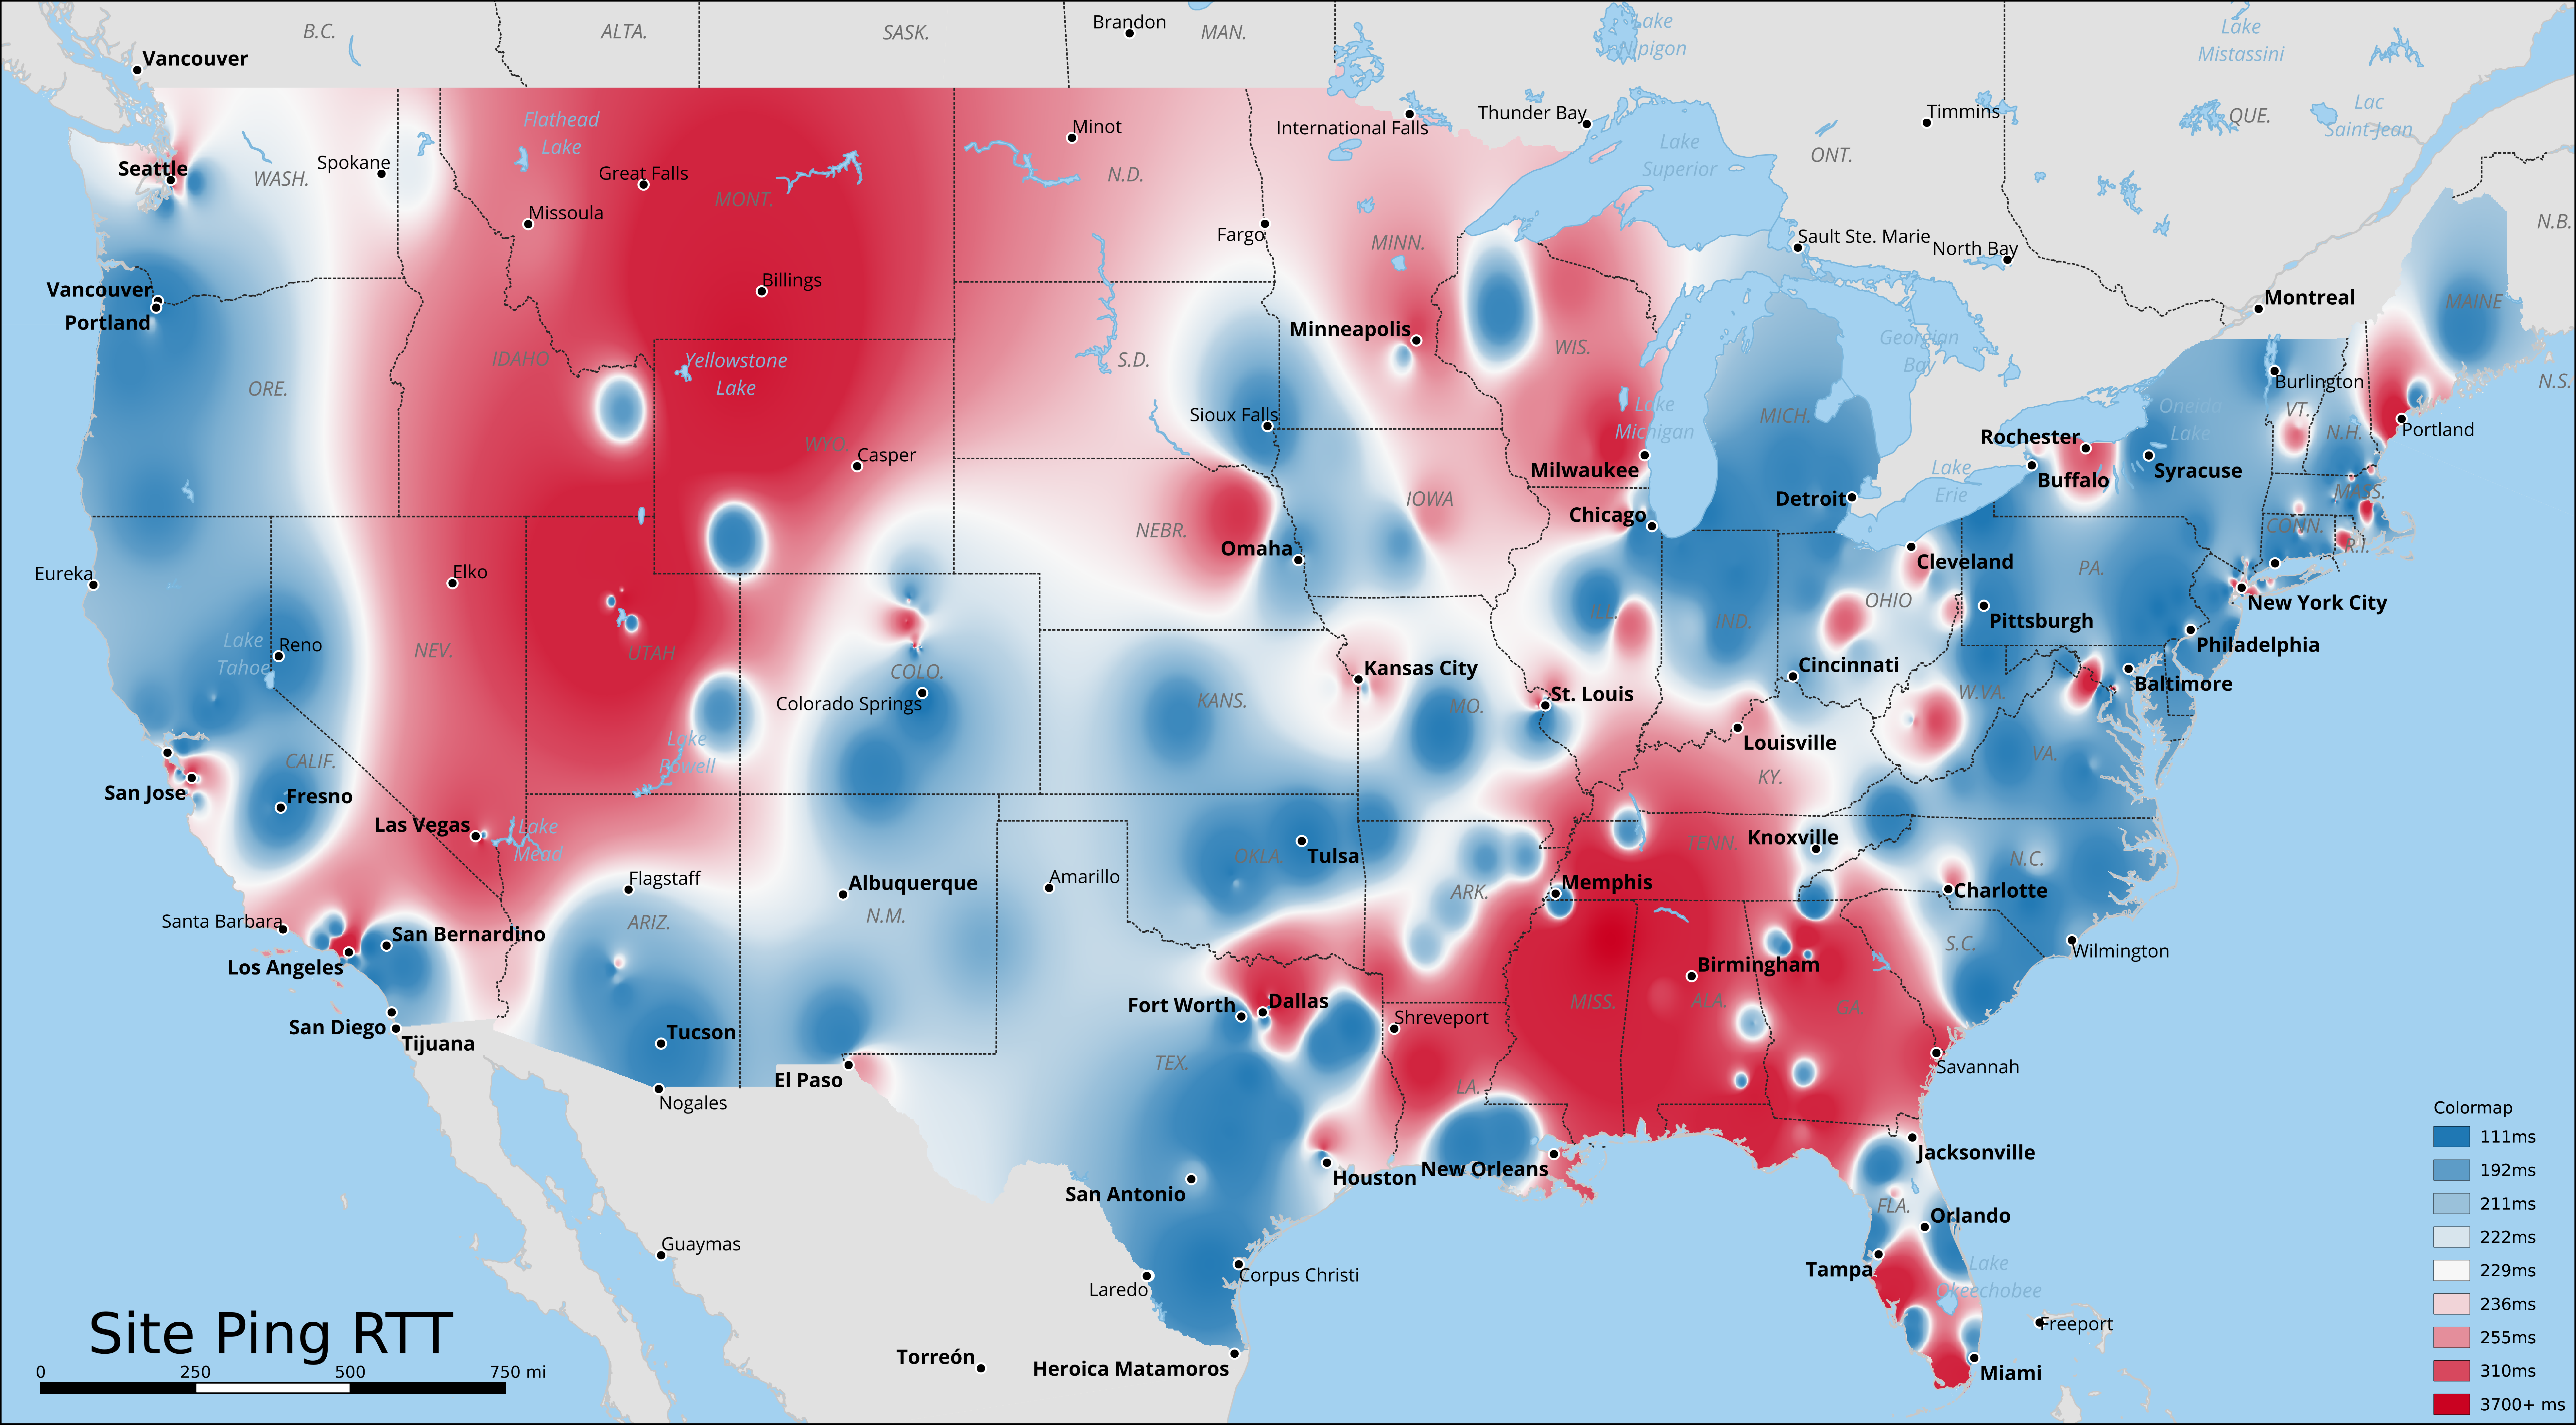
\includegraphics[width=0.75\textwidth]{images/siteping/site_ping_rtt_idw.png}
    \caption{Final heat map} % you've been visited by the latex fairy
    \label{fig:siteping_heatmap}
\end{figure}
